\section{Grundlegender Anwendungsfall (Geschäftsvorfall)}

\begin{tcolorbox}
    Ein \textbf{Grundlegender Anwendungsfall} (auch \textit{Essential Use Case} oder \textit{Geschäftsvorfall /Geschäftsanwendungsfall}\footnote{
        \textit{Geschäftsanwendungsfall} bspw. bei \cite[101]{Oes05}
    }) beschreibt unter vollständigem Verzicht auf Details der Technik oder der späteren Nutzung, wie der Endnutzer mit dem System umgeht und wie das System darauf reagieren soll (vgl. \cite[68]{Wed09}).
\end{tcolorbox}

\textit{Ambler} definiert den \textbf{Essential Use Case} als
\blockquote[{\cite[184]{Amb04}}]{
    A simplified, abstract, generalized use case that captures the intentions of a user
    in a technology and implementation independent manner
}


\begin{figure}
    \centering
    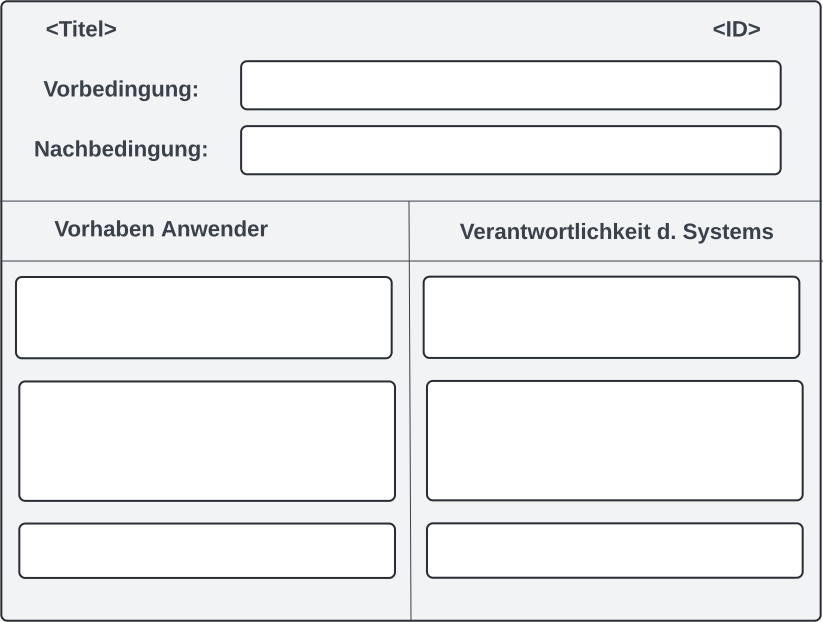
\includegraphics[scale=0.3]{chapters/Anhang/CheatSheets/img/essentialusecasetemplate}
    \caption{Vorlage zur Erstellung eines \textbf{Essential Use Case}. (Quelle: in Anlehnung an \cite[Figure 2]{CL01})}
    \label{fig:essentialusecasetemplate}
\end{figure}